%!TEX program = xelatex
%使用xelatex,使用unicode,对中文支持的最好.记得文档另存为uft-8格式.

\documentclass[10pt,a4paper,titlepage]{article} %默认字体大小,页面大小(a4),标题单独一页
\usepackage{fontspec}   %引入设置字体的包
\usepackage{xeCJK}  %使用中文环境的包,还有一个是CJK,未知
\usepackage{graphicx}
\usepackage{subfigure}


\setmainfont{Times New Roman}   %英文字体
\setCJKmainfont[BoldFont=MicrosoftYaHei]{MicrosoftYaHei}      %中文字体`'


\title{资源管理器概要设计}
\author{作者:李辉}
\date{2018.6.7}

\begin{document}
	\maketitle
	\newpage

	\begin{flushleft}
	\section{概述(Introduction)}
		\subsection{目的(Purpose)}
		本文主要是TVOS中间间的子模块资源管理器模块的概要设计,重点描述了如何
		通过资源管理器使用,管理独占的硬件资源,以满足PIP等多个播放器同时播放
		的需求场景。
		\subsection{范围(Scope)}
		本文主要包括RM的接口设计及使用场景设计,由于模块本身较小,实现较简
		单,不再做内部分解设计。
		\subsection{略略语(Acronyms \& Definaitions)}
		\begin{tabular}{|c|c|c|}
		\hline
		缩略语&英文&中文解释\\
		\hline
		TVOS&TVOS&TCL智能电视中间件系统\\
		\hline
		RM&Resource Manager&资源管理器,TVOS中间件的子模块。\\
		\hline
		\end{tabular}

		\subsection{参考(References)}
		SITA中间件概要设计DTVM中间件规范
		\subsection{发布范围}
		\begin{center}
		\begin{tabular}{|c|c|p{100pt}|c|}
		\hline
		序号&持有人角色&持有人姓名&发布日期\\
		\hline
		1&作者&李辉&2016.7.6\\
		\hline
		2&初评&樊二锋、赵德民、罗阳志、路惠明、付勇、林舜大、黄高波等&2016.7.8\\
		\hline
		\end{tabular}
		\end{center}
		\newpage
	\section{概要设计(High Level Design)}
		\subsection{系统需求 (System Requirements)}
			\begin{itemize}
        		\item 支持创建、删除资源管道
        		\item 实现像资源管道添加、删除资源
        		\item 支持申请、释放资源管道里的所有资源, 并协调资源管道间的资源冲突
        		\item 支持查询各硬件资源的状态
        		\item 支持关注资源管道的资源使用情况,并修改资源管道间的资源冲突解决策略
     		\end {itemize}
			\begin{figure}[h]
				\centering
				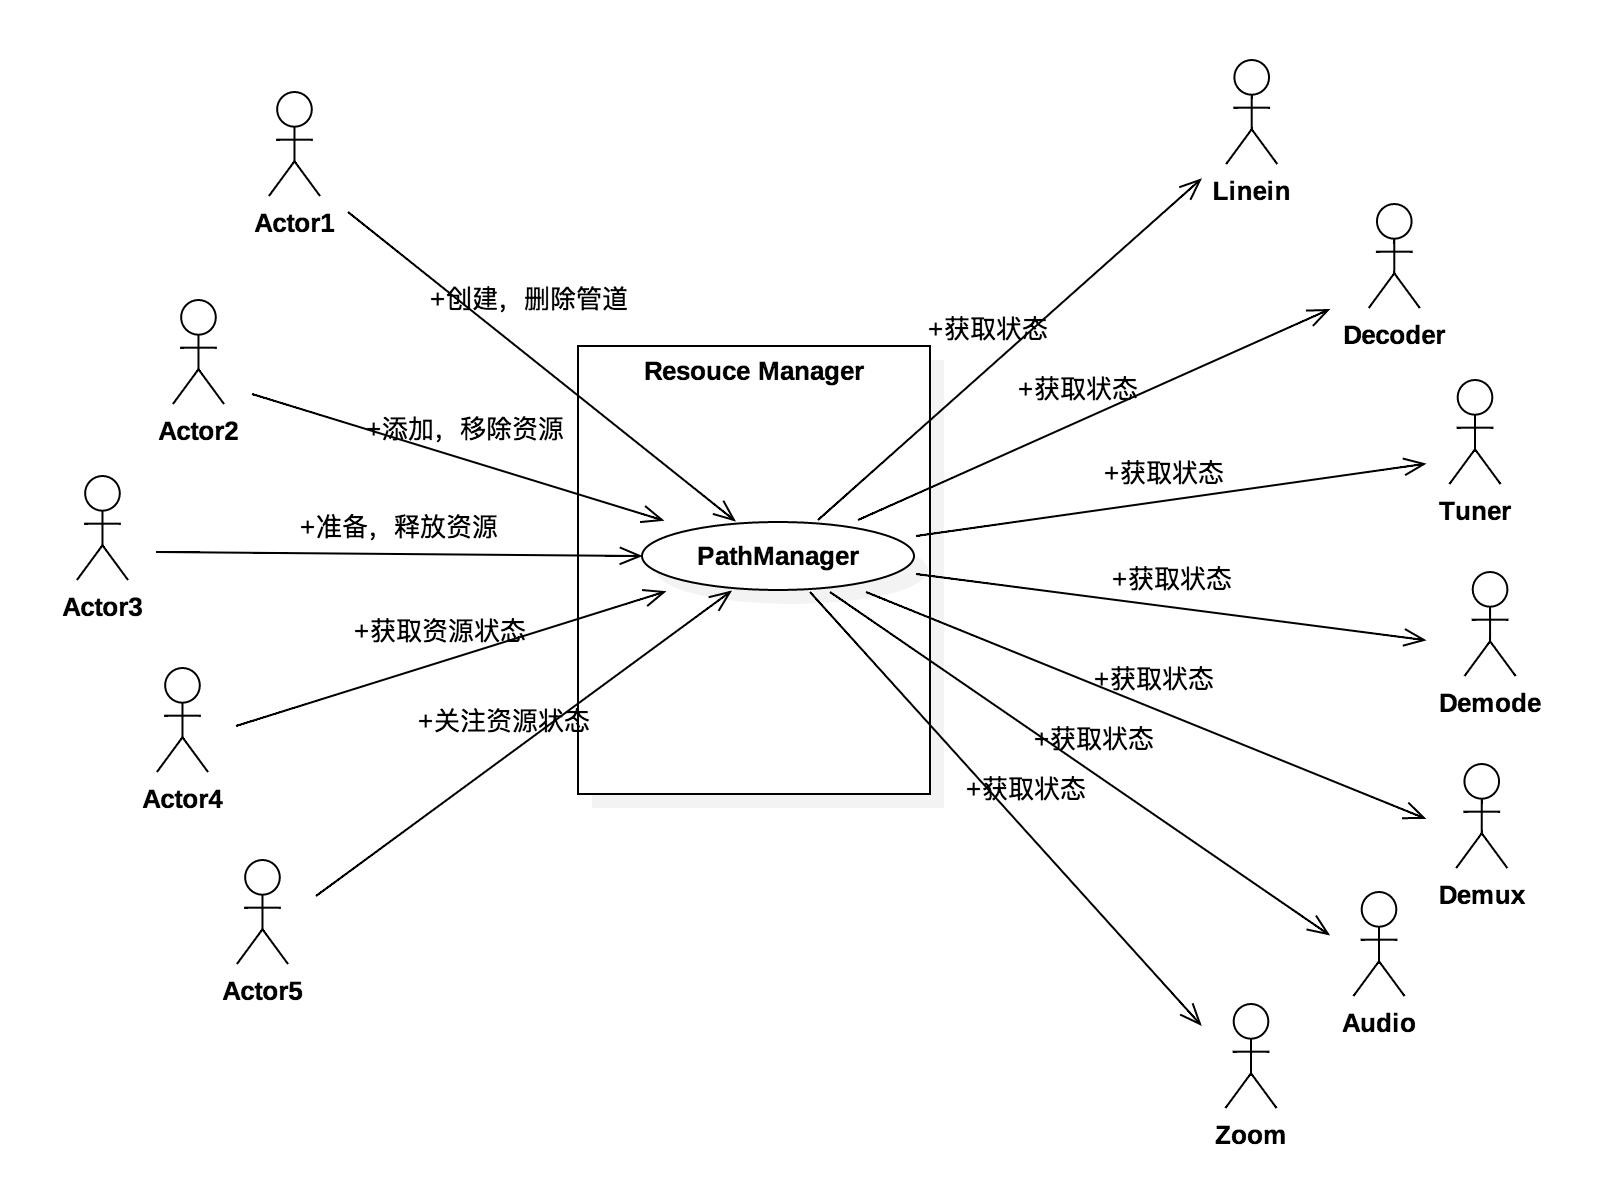
\includegraphics[width=7cm,height=8cm]{2.1}
			\end{figure}
\centerline{{图 2.1: 资源管理器系统需求概述}}
         \subsection{设计约束 (Design Constraint)}
         \subsubsection{需求约束}
         不得对现有架构做过大的调整,特别是涉及到 T-HAL 接口重定义会产生极大的工作量。
         \subsubsection{隐含约束}
         资源冲突解决策略是一个复杂而庞大的工程,需要根据后续应用场景的丰富逐步完善。
		 因此 RM 需支持先使用简单策略(如后来优先),并支持应用后续根据使用场景逐步扩展细化策略。
		\newpage
	\end{flushleft}

\end{document}
